\title{Survivability in slasher movies: \\abstinence and gender}
\author{Pedro Henrique Luz de Araujo}
\date{\today}

\documentclass[12pt]{article}
\usepackage{graphicx}
\usepackage{booktabs}
\usepackage{tabularx}

\begin{document}
\maketitle

\begin{abstract}
This is the paper's abstract \ldots
\end{abstract}

\section{Introduction}
Problem: Does gender influence survivability in slasher movies? Does sexual activity? How do they interact?

\paragraph{Outline}
The remainder of this article is organized as follows.
Section~\ref{previous work} gives account of previous work.
Our new and exciting results are described in Section~\ref{results}.
Finally, Section~\ref{conclusions} gives the conclusions.

\section{Data}\label{data}
The data\footnote{Welsh, A. On the Perils of Living Dangerously in the Slasher Horror Film: Gender Differences in the Association Between Sexual Activity and Survival. Sex Roles 62, 762–773 (2010). https://doi.org/10.1007/s11199-010-9762-x} include the survival status of 485 characters from 50 North American slasher films released between 1960 and 2009 randomly sampled from the Internet Movie Database (IMDb)\footnote{https://www.imdb.com/.}. The population was selected using keywords associated with the slasher genre; i.e.\ slasher, masked killer, gore, among others.

As explanatory variables we have the ``Gender'' and ``Involvement in Sexual Activity''. The first is taken to be the biological sex of the character, while the second is true if the character is involved with full or partial nudity or extended physical intimacy with another character. Only characters that suffered some kind of physical aggression are included. This was measured by undergraduate students. Refer to the original paper for a more detailed explanation of the data acquisition process.

45.77\% Female
32.37\% sexual activity
37.39\% Female have sexual activity
28.14\% Male have sexual activity
17.53\% Survival Rate
52.87\% Sexual activity are female
22.52\$ Female survive
13.30\% Men survive

\begin{table}
    \centering
    \footnotesize
    \caption{Sexual activity across genders.}
    \label{tab:sexXgender}
    \begin{tabularx}{\textwidth}{X X X r}
        \toprule
        & \multicolumn{2}{c}{Gender} & Total \\
        \cmidrule{2-3}
        & Male & Female & \\
        \midrule 
        Presence & 74 & 83 & 157 \\
        Absence & 189 & 139 & 328\\  
        Total & 263 & 222& 485\\  
        \bottomrule
       \end{tabularx}
\end{table}



\begin{figure}[h]
    \caption{Relationships between variables}
    \centering
    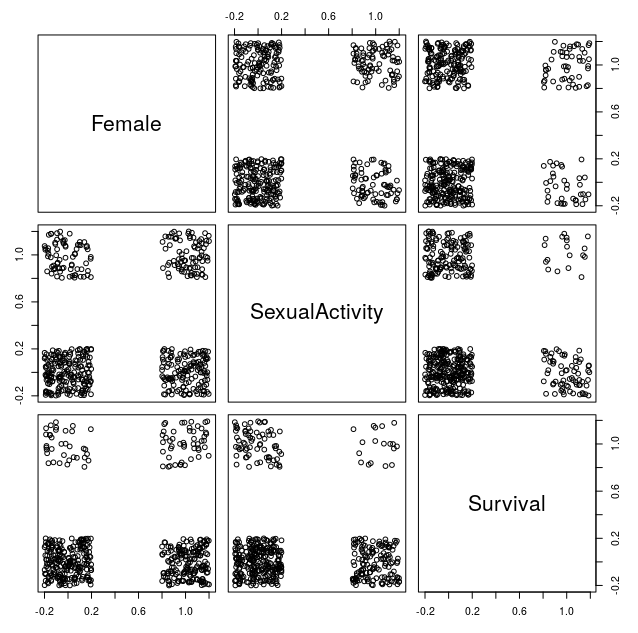
\includegraphics[width=0.5\textwidth]{media/pairs.png}
    \end{figure}

\section{Model}
Since we have a binary response variable, a logistic regression method is appropriate.

\section{Results}\label{results}
In this section we describe the results.

\section{Conclusions}\label{conclusions}
We worked hard, and achieved very little.

\end{document}